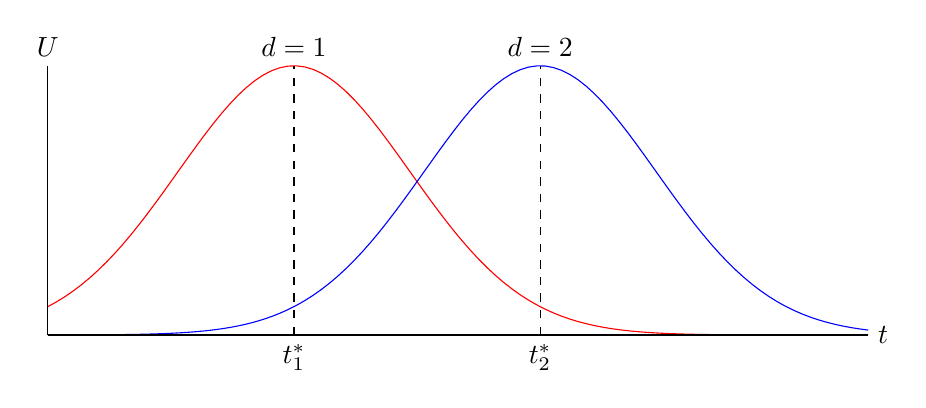
\begin{tikzpicture}[
declare function={ normal(\x,\u,\s) = 1/(\s*sqrt(2*pi))*exp(-pow((\x-\u),2)/(2*\s));
                 },
]

\begin{axis}[
  no markers, domain=-2:8, samples=100,
  axis lines*=left, 
  xlabel=$t$, ylabel=$U$,
  every axis y label/.style={at={(ticklabel* cs:1)}, anchor=south,},
  every axis x label/.style={at=(current axis.right of origin),anchor=west},
  height=5cm, width=12cm,
  xtick=\empty, ytick=\empty,
  enlargelimits=false, clip=false, axis on top,
  grid = major
] % extend the axes a bit to the right and t
    						
\addplot[mark=none, red]  {normal(x,1,2)};
\addplot[mark=none, blue] {normal(x,4,2)};
\pgfmathsetmacro\meanone{normal(1,1,2)}
\pgfmathsetmacro\meantwo{normal(4,4,2)}
\draw[dashed] (axis cs:1,0) -- (axis cs:1,\meanone);
\draw[dashed] (axis cs:4,0) -- (axis cs:4,\meantwo);
\node[below] at (axis cs:1,0){$t^*_1$};
\node[below] at (axis cs:4,0){$t^*_2$};
\node[above] at (axis cs:1,\meanone){$d=1$};
\node[above] at (axis cs:4,\meantwo){$d=2$};
\end{axis}
\end{tikzpicture}           